\chapter{Demystifying the Higgs Boson}

These companion notes follow Leonard Susskind's lecture on the Higgs boson and are curated by LazyingArt LLC. The lecture is deliberately narrower than the surrounding public excitement: its purpose is not to repeat the newspaper claims about the origin of the universe, but to explain, in the space of one hour, the nuts and bolts of Higgs physics. The argument unfolds in modules. It begins with quantization, fields, and vacuum structure; it then turns to spontaneous symmetry breaking in field space; only after that does it ask why the particles of the Standard Model would otherwise be massless, and how the Higgs mechanism changes that conclusion. Throughout, the order matters: the bowl and the sombrero come first, the Standard Model comes second, and the Higgs boson itself appears only after the condensate and the ``Ziggs'' mechanism are already in place.

\section{Aim of the Lecture}

Susskind opens by refusing the standard public script. The Higgs boson is certainly important, and the excitement surrounding its discovery is justified, but that is not the task he sets himself for the evening. His task is narrower and more technical: not why the Higgs is culturally momentous, but how Higgs physics actually works.

He also pauses almost immediately to credit Fran\c{c}ois Englert and to remind the audience that the phenomenon is historically broader than the single word ``Higgs.'' From time to time he mentions the Braut--Englert--Higgs effect, even though in the lecture he mostly follows common usage and says ``Higgs effect.'' That opening sets the tone correctly. The lecture is simplifying for pedagogy, but it is not trying to erase the real structure or the real history.

The lecture is therefore built as a staged construction. Higgs physics, Susskind insists, is a highly quantum-mechanical effect, but he does not give a full course in quantum theory. He isolates only the ingredients he actually needs, and each later step is motivated by the one before it.

\section{Minimal Prerequisites: Quantization, Fields, and Vacuum}

After the brief interruption near the beginning, the technical development restarts in a cleaner form. Susskind says that for tonight's purposes quantum mechanics contributes two facts. The first is quantization, and the example he chooses is angular momentum:
\begin{equation}
L=n\hbar,\qquad n=0,\pm1,\pm2,\dots
\end{equation}
The point is not the full theory of angular momentum, but the simpler fact that some physical quantities do not vary continuously. They come in discrete units.

The second quantum fact, which he postpones for a few minutes, is the uncertainty principle. Before returning to it, he introduces the classical notion of a field.

\begin{definition}
A field is a physical quantity specified at each point of space and time. In the language of the lecture, electric, magnetic, and gravitational fields are standard examples. The vacuum is the state of lowest energy, and it need not coincide with vanishing field values.
\end{definition}

This last remark is already a preparation for the Higgs story. Empty space is often imagined as a place where all fields vanish, but that is only a common expectation, not a universal requirement. One may perfectly well imagine a world in which empty space is permeated by a field, just as one may imagine an electric field established by capacitor plates so distant that, for practical purposes, the world simply seems to contain that field.

Susskind's next move is to think of energy as a function of field value. If the energy is minimized at some field configuration, then that configuration is the vacuum. If the field is locally displaced and allowed to oscillate, the oscillation is quantized. Those quanta are the particles. In the lecture's repeated phrase, particles are quanta of field vibrations.

\section{Field-Space Potentials and the Bowl Analogy}

The first real mathematical picture of the lecture is an energy landscape. For a single field component, the ordinary minimum may be modeled schematically by
\begin{equation}
V(\phi)\propto \phi^{2}.
\end{equation}
This is not a literal board equation. It is the simplest mathematical model of the bowl-shaped geometry Susskind draws and discusses.

He then asks the audience to imagine more than one field component. In the lecture he says one may think of ``\(\phi\) and \(\phi'\).'' It is convenient to normalize that to a two-component field \((\phi_{1},\phi_{2})\). Then the potential is a surface over field space rather than over ordinary space:
\begin{equation}
V(\phi_{1},\phi_{2})\approx a(\phi_{1}^{2}+\phi_{2}^{2}),\qquad a>0.
\end{equation}
The important point is geometric. No matter in which direction the field is displaced from the origin, energy increases. The potential is rotationally symmetric in field space.

\begin{remark}
The blackboard images in this section display geometry rather than algebra. The labels \(V\), \(\phi\), \(\phi_{1}\), and \(\phi_{2}\) are added here for mathematical clarity; they are not visible on the board itself.
\end{remark}

\begin{figure}
\centering

\includegraphics[width=0.78\textwidth]{lecture_144_figure_02.png}
\caption{Susskind's board sketch of the symmetric bowl together with the hat analogy used to emphasize rotational symmetry in field space.}
\end{figure}

\begin{figure}
\centering
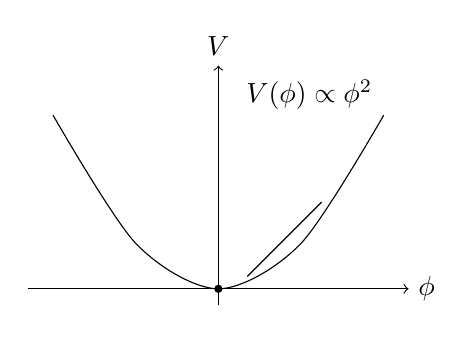
\begin{tikzpicture}[scale=1.05]
\draw[->] (-2.3,0) -- (2.3,0) node[right] {$\phi$};
\draw[->] (0,-0.2) -- (0,2.7) node[above] {$V$};
\draw plot[smooth] coordinates {(-2.0,2.1) (-1.0,0.55) (0,0) (1.0,0.55) (2.0,2.1)};
\fill (0,0) circle (0.05);
\draw (0.35,0.15) -- (1.25,1.05);
\node at (1.1,2.35) {$V(\phi)\propto \phi^2$};
\end{tikzpicture}
\caption{Editorial reconstruction of the ordinary bowl potential suggested by the board sketch. The diagonal line is retained only as a guide to the lecture's geometry and may be read as a displacement direction or a slice through field space.}
\end{figure}

At this stage Susskind wants more than the minimum itself. He wants motion around it. If the field is displaced from the center and then set moving in a circle in field space, that motion carries an internal angular momentum. It is not angular momentum in ordinary space, but it behaves analogously: it is quantized, and Susskind uses it as the prototype of charge:
\begin{equation}
L_{\mathrm{int}}=n\hbar.
\end{equation}
The lecture does not turn this into a precise identity between electric charge and \(L_{\mathrm{int}}\), but it insists on the physical way of thinking: a charged excitation is naturally viewed as a field that rotates in an internal space.

That point is essential because the next construction will change the vacuum geometry while preserving the same internal rotational idea.

\section{The Mexican Hat, the Broken-Symmetry Vacuum, and the Condensate}

Susskind now reaches for the hat and turns it over. In the ordinary bowl the minimum sits at the center. In the inverted hat, the center becomes unstable and the minimum is pushed out to the brim. A standard analytic model of that geometry is
\begin{equation}
V(\phi_{1},\phi_{2})=\lambda\bigl(\phi_{1}^{2}+\phi_{2}^{2}-v^{2}\bigr)^{2},
\end{equation}
with minima satisfying
\begin{equation}
\phi_{1}^{2}+\phi_{2}^{2}=v^{2}.
\end{equation}
Thus the vacuum is no longer at zero field. The field sits somewhere on a circle of degenerate minima, and a chosen point on that circle may be parameterized as
\begin{equation}
(\phi_{1},\phi_{2})=v(\cos\theta,\sin\theta).
\end{equation}

\begin{figure}
\centering

\includegraphics[width=0.72\textwidth]{lecture_144_figure_03.png}
\caption{The lecture's transition to the sombrero or Mexican-hat potential. The board shows the central peak and surrounding trough, while the hat remains part of the live analogy.}
\end{figure}

\begin{figure}
\centering
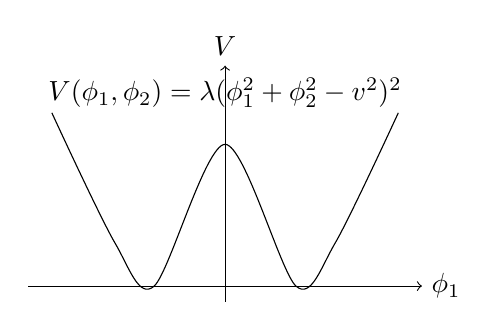
\begin{tikzpicture}[scale=1.0]
\draw[->] (-2.5,0) -- (2.5,0) node[right] {$\phi_1$};
\draw[->] (0,-0.2) -- (0,2.8) node[above] {$V$};
\draw plot[smooth] coordinates {(-2.2,2.2) (-1.4,0.55) (-0.9,0.0) (0,1.8) (0.9,0.0) (1.4,0.55) (2.2,2.2)};
\node at (0,2.45) {$V(\phi_1,\phi_2)=\lambda(\phi_1^2+\phi_2^2-v^2)^2$};
\end{tikzpicture}
\caption{Cross-sectional reconstruction of the Mexican-hat potential. The board provides the geometry; the formula is a cautious standard completion.}
\end{figure}

This geometric change immediately alters the dynamics. In the ordinary bowl, rotational motion requires first displacing the field from the center and then pushing it around. On the brim of the Mexican hat, by contrast, the field can move around the trough without climbing the potential. The radius stays essentially fixed while only the angular position changes. Charge-like motion has become cheap.

\begin{figure}
\centering

\includegraphics[width=0.72\textwidth]{lecture_144_figure_04.png}
\caption{The later board state in which a specific point on the trough is marked. This is the lecture's move from a degenerate set of minima to a chosen vacuum.}
\end{figure}

\begin{figure}
\centering
\begin{tikzpicture}[scale=1.1]
\draw[->] (-2.2,0) -- (2.2,0) node[right] {$\phi_{1}$};
\draw[->] (0,-2.2) -- (0,2.2) node[above] {$\phi_{2}$};
\draw (0,0) circle (1.5);
\fill (1.06,1.06) circle (0.06);
\node[right] at (1.12,1.06) {$v(\cos\theta,\sin\theta)$};
\node at (0.15,1.85) {$\phi_1^2+\phi_2^2=v^2$};
\end{tikzpicture}
\caption{Reconstruction of the vacuum manifold in field space. The chosen point is not read from a board label; it is the mathematical completion of the marked point visible in the screenshot.}
\end{figure}

At first one might draw a classical conclusion: the true vacuum should simply pick one point on the rim and remain at rest there. Susskind's next move is to explain why quantum mechanics blocks that over-simple picture. The uncertainty principle enters in the schematic form he actually uses:
\begin{equation}
\Delta x\,\Delta p \gtrsim \hbar.
\end{equation}
Applied to the brim of the Mexican hat, the same logic says that if the field is sharply localized at one angular position, then the conjugate angular motion must be uncertain. In the language of this lecture one may formalize that as
\begin{equation}
\Delta\theta\,\Delta L_{\mathrm{int}} \gtrsim \hbar.
\end{equation}
So the field cannot be both sharply fixed on the rim and sharply free of angular motion or charge.

This is the point where the lecture turns from a classical symmetry-breaking picture into a genuinely quantum one. Empty space is no longer described as a state with a definite charge; it becomes a state with indefinite charge content. Susskind's operational characterization is striking: if one adds one unit of charge, or removes one, nothing essential changes. The state is already so indefinite that such an operation merely relabels it. That is what he calls a condensate.

He pushes the point further by saying that if this were ordinary electric charge, then a region of empty space would contain a totally uncertain amount of charge. One should not try to visualize that literally. The point is operational: charge is so uncertain that inserting one more unit or removing one does not change the state. This is why the lecture ends module number one with superconductors. A superconductor is not a metaphor here; it is the concrete physical example that makes the condensate idea feel less exotic.

\section{Standard Model Inventory and Why Mass Is a Puzzle}

Only after the condensate story is in place does Susskind announce module number two: the Standard Model. The transition matters. The first module has shown how a condensate can exist; the second asks which particles need such a condensate in order to become massive.

He begins with a scale argument. Elementary-particle masses could in principle range all the way up to the Planck scale before black-hole physics intervenes, yet the known particles sit far down near the bottom of that enormous range. In the lecture's 2012 language, even the heaviest known elementary particle lies only around \(10^{-17}\) of the Planck mass.

He then inventories the particles. The fermions are the matter particles: electrons, neutrinos, quarks, and their heavier relatives. The bosons are the force carriers: the photon \(\gamma\), the gluon \(g\), and the weak bosons \(W\) and \(Z\). Susskind presents the Standard Model not as a static list but as a set of basic emission processes:
\begin{align}
e &\to e+\gamma,\\
q &\to q+g,\\
f &\to f+Z.
\end{align}
The first is the emission of a photon by an electrically charged particle, the second the emission of a gluon by a quark, and the third the emission of a \(Z\) by any fermion carrying the relevant weak quantum number.

\begin{figure}
\centering
\begin{tikzpicture}[scale=1.0]
\draw (0,0) -- (1.5,0);
\draw (1.5,0) -- (3.0,0);
\draw (1.5,0) -- (2.6,0.9);
\node at (0.45,0.25) {$e$};
\node at (2.45,-0.25) {$e$};
\node at (2.45,1.15) {$\gamma$};

\draw (4.2,0) -- (5.7,0);
\draw (5.7,0) -- (7.2,0);
\draw (5.7,0) -- (6.8,0.9);
\node at (4.65,0.25) {$q$};
\node at (6.65,-0.25) {$q$};
\node at (6.55,1.15) {$g$};

\draw (8.4,0) -- (9.9,0);
\draw (9.9,0) -- (11.4,0);
\draw (9.9,0) -- (11.0,0.9);
\node at (8.85,0.25) {$f$};
\node at (10.85,-0.25) {$f$};
\node at (10.75,1.15) {$Z$};
\end{tikzpicture}
\caption{Transcript-based reconstruction of the three emission processes Susskind uses to summarize the Standard Model.}
\end{figure}

The puzzle now becomes sharp. If this were all there was, then the particles in this bare Standard Model would be massless. Susskind makes the point first for the bosons: the photon is massless, and the same style of gauge theory would also leave the gluon and the \(Z\) massless. But he immediately broadens the question: why should the fermions also come out massless, and what extra ingredient changes that answer?

\section{How Fields Affect Mass, and Why Not All Mass Is Higgs Mass}

Before giving the Higgs mechanism proper, Susskind inserts two detours. The first is constructive: a background field can shift energies and therefore masses. The second is restrictive: much of the mass in nature has nothing to do with Higgs physics.

The constructive detour is the water molecule. Treated crudely as a dipole with one positive end and one negative end, it has two opposite orientations with equal mass in empty space. Once it is placed in a uniform electric field, that degeneracy is lifted. If the dipole moment has magnitude \(d\) and the field has magnitude \(E\), then the two orientations receive opposite energy shifts:
\begin{align}
\Delta E_{\uparrow} &= -dE,\\
\Delta E_{\downarrow} &= +dE.
\end{align}
By
\begin{equation}
E=mc^{2},
\end{equation}
this becomes a mass splitting:
\begin{equation}
m_{\downarrow}-m_{\uparrow}
=
\frac{\Delta E_{\downarrow}-\Delta E_{\uparrow}}{c^{2}}
=
\frac{2dE}{c^{2}}.
\end{equation}
This is the lecture's explicit worked example of a field changing mass.

\begin{figure}
\centering
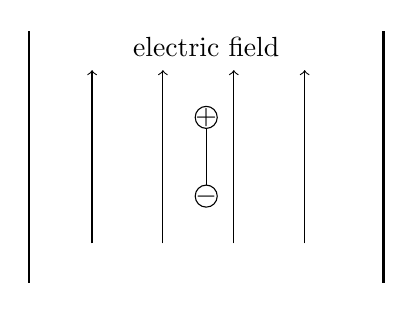
\begin{tikzpicture}[scale=1.0]
\draw[line width=1pt] (0,0) -- (0,3.2);
\draw[line width=1pt] (4.5,0) -- (4.5,3.2);
\draw[->] (0.8,0.5) -- (0.8,2.7);
\draw[->] (1.7,0.5) -- (1.7,2.7);
\draw[->] (2.6,0.5) -- (2.6,2.7);
\draw[->] (3.5,0.5) -- (3.5,2.7);
\draw (2.25,1.1) circle (0.14);
\draw (2.25,2.1) circle (0.14);
\node at (2.25,1.1) {$-$};
\node at (2.25,2.1) {$+$};
\draw (2.25,1.24) -- (2.25,1.96);
\node at (2.25,3.0) {electric field};
\end{tikzpicture}
\caption{Transcript-based reconstruction of the capacitor-field and water-dipole example. The point of the example is an energy shift between two internal configurations, not drag.}
\end{figure}

Two things matter here. First, the field changes energy and hence mass. Second, it does so without introducing friction. This is why Susskind rejects the popular ``molasses'' analogy. The vacuum is not sticky. The molecule does not get slowed by drag; it passes through the field with no net force, while the two internal configurations simply carry different energies.

He then retells the same example in particle language. An electric field may be viewed as a condensate of photons. The water molecule continually emits and reabsorbs photons into that condensate. Since a condensate is a background for which adding or removing one quantum does not appreciably change the state, the emitted photon may simply disappear into the condensate. That is what the terminating cross is meant to represent in the lecture.

\begin{figure}
\centering
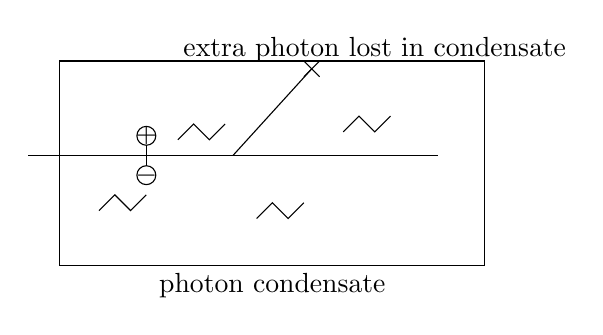
\begin{tikzpicture}[scale=1.0]
\draw (0,0.4) rectangle (5.4,3.0);
\draw (0.5,1.1) -- (0.7,1.3) -- (0.9,1.1) -- (1.1,1.3);
\draw (1.5,2.0) -- (1.7,2.2) -- (1.9,2.0) -- (2.1,2.2);
\draw (2.5,1.0) -- (2.7,1.2) -- (2.9,1.0) -- (3.1,1.2);
\draw (3.6,2.1) -- (3.8,2.3) -- (4.0,2.1) -- (4.2,2.3);
\draw (-0.4,1.8) -- (2.2,1.8);
\draw (2.2,1.8) -- (4.8,1.8);
\draw (2.2,1.8) -- (3.2,2.9);
\draw (3.10,2.80) -- (3.30,3.00);
\draw (3.10,3.00) -- (3.30,2.80);
\draw (1.1,1.55) circle (0.12);
\draw (1.1,2.05) circle (0.12);
\node at (1.1,1.55) {$-$};
\node at (1.1,2.05) {$+$};
\draw (1.1,1.67) -- (1.1,1.93);
\node at (2.7,0.15) {photon condensate};
\node at (4.0,3.15) {extra photon lost in condensate};
\end{tikzpicture}
\caption{Transcript-based reconstruction of the field-as-condensate picture. The background electric field is reinterpreted as a condensate of photons into which an emitted photon may disappear.}
\end{figure}

Susskind then turns the example around and asks a more basic question: does an object need the Higgs phenomenon in order to have mass at all? The answer is no. A box filled with trapped radiation behaves as a massive object simply because it stores energy:
\begin{equation}
m_{\text{box}}=\frac{E_{\text{contained}}}{c^{2}}.
\end{equation}
That observation is immediately applied to the proton. A proton is made of quarks and many gluons, and most of its mass comes from the kinetic and binding energy of those constituents rattling around inside the hadronic ``box.'' In the lecture's estimate, even if the quarks and gluons were massless, the proton would lose only of order one percent of its mass. Higgs physics is therefore not an explanation of all mass in nature. It is a very specific explanation of the masses of the Standard Model fermions and weak bosons.

\section{Electron Chirality, Ziggs, the Higgs Boson, and 2012 Phenomenology}

Having cleared away those detours, Susskind narrows everything to the electron. He does not develop the full Dirac equation, but he isolates one feature of Dirac theory that is enough for the lecture: an electron has left-handed and right-handed chiral states, and the mass is tied to the rate at which it flips between them. In standard compact notation, that statement is encoded by the Dirac mass term
\begin{equation}
m_{D}\bar\psi\psi
=
m_{D}\bigl(\bar\psi_{L}\psi_{R}+\bar\psi_{R}\psi_{L}\bigr).
\end{equation}
This is not a board equation, but it is the clean mathematical form of Susskind's verbal summary that mass is the rate of left-right flipping.

\begin{figure}
\centering
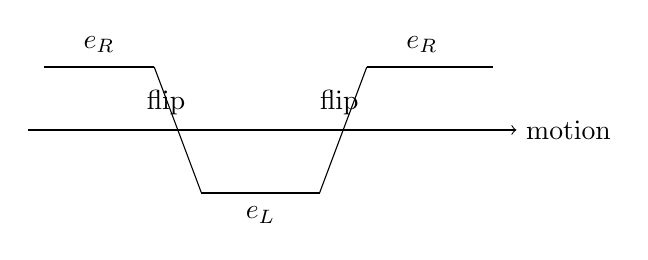
\begin{tikzpicture}[scale=1.0]
\draw[->] (0,0) -- (6.2,0) node[right] {motion};
\draw (0.2,0.8) -- (1.6,0.8);
\draw (1.6,0.8) -- (1.9,0.0);
\draw (1.9,0.0) -- (2.2,-0.8);
\draw (2.2,-0.8) -- (3.7,-0.8);
\draw (3.7,-0.8) -- (4.0,0.0);
\draw (4.0,0.0) -- (4.3,0.8);
\draw (4.3,0.8) -- (5.9,0.8);
\node at (0.9,1.08) {$e_{R}$};
\node at (2.95,-1.08) {$e_{L}$};
\node at (5.0,1.08) {$e_{R}$};
\node at (1.75,0.35) {flip};
\node at (3.95,0.35) {flip};
\end{tikzpicture}
\caption{Transcript-based reconstruction of Susskind's picture of mass as repeated left-right chirality flipping.}
\end{figure}

If the electron were strictly massless and moving at the speed of light, then in the lecture's language nothing internal could happen to it, so there would be no flipping. A massless electron would remain purely left-handed or purely right-handed. Why, then, is the flip forbidden in the bare Standard Model?

The answer enters through the \(Z\) boson. Susskind introduces a second conserved quantity, distinct from electric charge, associated with \(Z\)-boson emission. Instead of using the standard but awkward name, he renames it ``zilch.'' The key assignments in the lecture are
\begin{equation}
z(e_{L})=1,\qquad z(e_{R})=0.
\end{equation}
Left-handed and right-handed electrons have the same ordinary electric charge, but they do not have the same zilch. So a direct chirality flip would change a conserved quantity:
\begin{equation}
e_{L}\not\to e_{R}\qquad \text{in the bare theory.}
\end{equation}
That is Susskind's explanation of why the electron is massless in the stripped-down Standard Model.

The cure is the new ingredient that he pointedly does not yet call the Higgs boson. It is the ``Ziggs'' boson, a field that forms a condensate carrying indefinite zilch. Then the forbidden transition becomes possible in two steps:
\begin{align}
e_{L} &\to e_{R}+\mathrm{Ziggs},\\
e_{R}+\mathrm{Ziggs} &\to e_{L}.
\end{align}
Because the condensate does not change when one Ziggs quantum is added or removed, the emitted Ziggs can disappear into the condensate, or one can be pulled back out of it, without changing the vacuum in any essential way. Left-right mixing is restored, and with it the fermion mass.

\begin{figure}
\centering
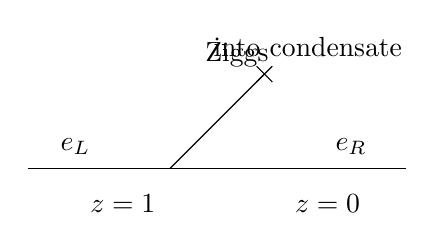
\begin{tikzpicture}[scale=1.0]
\draw (0,0) -- (1.8,0);
\draw (1.8,0) -- (4.8,0);
\draw (1.8,0) -- (3.0,1.2);
\draw (2.9,1.1) -- (3.1,1.3);
\draw (2.9,1.3) -- (3.1,1.1);
\node at (0.6,0.28) {$e_{L}$};
\node at (4.1,0.28) {$e_{R}$};
\node at (2.65,1.45) {$\mathrm{Ziggs}$};
\node at (1.2,-0.45) {$z=1$};
\node at (3.8,-0.45) {$z=0$};
\node at (3.55,1.55) {into condensate};
\end{tikzpicture}
\caption{Transcript-based reconstruction of the electron-mass mechanism in the lecture's own language. The electron flips chirality by emitting or absorbing a Ziggs quantum that is lost in the condensate.}
\end{figure}

Susskind immediately carries the same logic over to the \(Z\) boson. Since the Ziggs carries zilch and can emit a \(Z\), the \(Z\) can exchange zilch with the condensate through the Ziggs sector and thereby behave as a massive particle. In the lecture's emphasis, this is the Braut--Englert--Higgs phenomenon proper: the \(Z\) boson getting a mass. Had there been an analogous condensate for ordinary electric charge, the photon too would have become massive.

\begin{figure}
\centering
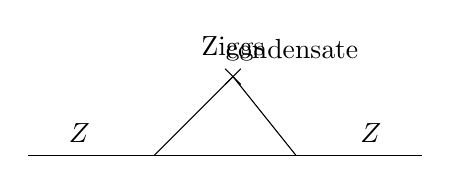
\begin{tikzpicture}[scale=1.0]
\draw (0,0) -- (5.0,0);
\draw (1.6,0) -- (2.6,1.0);
\draw (3.4,0) -- (2.6,1.0);
\draw (2.5,0.9) -- (2.7,1.1);
\draw (2.5,1.1) -- (2.7,0.9);
\node at (0.65,0.28) {$Z$};
\node at (4.35,0.28) {$Z$};
\node at (2.6,1.35) {$\mathrm{Ziggs}$};
\node at (3.35,1.35) {condensate};
\end{tikzpicture}
\caption{Transcript-based reconstruction of the analogous mechanism for the \(Z\)-boson mass. The boson mixes with condensate-supported Ziggs excitations.}
\end{figure}

At this point Susskind makes one of the lecture's most important distinctions. The Ziggs is not yet the Higgs boson. Indeed, he says explicitly that the Ziggs was, in effect, already discovered long ago through the observed properties of the \(Z\) boson. The Higgs boson is something else: not motion around the brim, but motion in and out of the brim. In standard field-theoretic notation one may capture that distinction by writing
\begin{equation}
\Phi(x)=(v+h(x))e^{i\theta(x)/v}.
\end{equation}
Here \(\theta(x)\) parameterizes the angular motion around the trough, while \(h(x)\) is the radial fluctuation. In the language of the lecture, \(\theta\) belongs to the Ziggs-like sector tied to the condensate, while \(h\) is the physical Higgs boson. Susskind then gives the same point in two pictures: \(h\) is either an oscillation in the magnitude of the field or a compression wave in the density of the condensate.

The short question period adds two clarifications that belong inside the main narrative. First, Susskind quotes the expectation value of the Higgs field as
\begin{equation}
v\approx 240\,\mathrm{GeV}.
\end{equation}
Second, he explains that different fermions have different coupling constants to the condensate, and that these couplings determine both the masses of the particles and the rates at which the Higgs decays into them. In standard notation, that lecture-level statement is summarized by
\begin{equation}
g_{Hff}\propto \frac{m_{f}}{v}.
\end{equation}
He is careful about the limit of the explanation: the coupling constants can be parameterized, but not explained from first principles in this lecture.

Susskind then asks what the Higgs boson itself does. He names it \(H\), and he emphasizes that one should read the basic diagram in both directions. As a decay process,
\begin{equation}
H\to f\bar f,
\end{equation}
and as a production process,
\begin{equation}
e^{+}e^{-}\to H.
\end{equation}
The second channel is, however, a very poor way to make Higgs bosons, because the electron is too light and therefore couples too weakly. The lecture's decisive phenomenological point is that heavier fermions couple more strongly.

That immediately singles out the top quark, which Susskind describes as roughly \(170\) proton masses in the lecture's numerical language. The top sector is the most favorable one for Higgs physics. At the same time, the Higgs with
\begin{equation}
m_{H}\approx 125\,\mathrm{GeV}
\end{equation}
is too light to decay into an on-shell top-antitop pair. The top quark instead enters through the loop that dominates Higgs production. The two central loop processes are
\begin{equation}
gg\to H,
\end{equation}
and the clean diphoton channel
\begin{equation}
H\to \gamma\gamma.
\end{equation}

\begin{figure}
\centering
\begin{tikzpicture}[scale=1.0]
\draw (0,0) -- (1.8,0);
\draw (1.8,0) -- (3.2,0.9);
\draw (1.8,0) -- (3.2,-0.9);
\node at (0.7,0.28) {$H$};
\node at (3.55,1.05) {$f$};
\node at (3.55,-1.05) {$\bar f$};
\end{tikzpicture}
\caption{Transcript-based reconstruction of Higgs decay into a fermion pair. The lecture emphasizes that heavier fermions are favored because they couple more strongly.}
\end{figure}

\begin{figure}
\centering
\begin{tikzpicture}[scale=0.95]
\draw (0,1.0) -- (1.2,1.0);
\draw (0,-1.0) -- (1.2,-1.0);
\draw (1.2,1.0) -- (2.2,0);
\draw (1.2,-1.0) -- (2.2,0);
\draw (1.2,1.0) -- (1.2,-1.0);
\draw (2.2,0) -- (3.5,0);
\node at (0.45,1.25) {$g$};
\node at (0.45,-1.25) {$g$};
\node at (3.9,0.25) {$H$};
\node at (1.55,0.25) {$t$};
\node at (1.55,-0.35) {$t$};

\draw (6.2,0) -- (7.4,0);
\draw (7.4,0) -- (8.4,1.0);
\draw (7.4,0) -- (8.4,-1.0);
\draw (8.4,1.0) -- (8.4,-1.0);
\draw (8.4,1.0) -- (9.6,1.0);
\draw (8.4,-1.0) -- (9.6,-1.0);
\node at (6.65,0.25) {$H$};
\node at (9.95,1.25) {$\gamma$};
\node at (9.95,-1.25) {$\gamma$};
\node at (8.75,0.25) {$t$};
\node at (8.75,-0.35) {$t$};
\end{tikzpicture}
\caption{Transcript-based reconstructions of the two loop processes emphasized near the end of the lecture: gluon-fusion production of the Higgs through a top loop, and diphoton decay through the same loop logic.}
\end{figure}

This is where the lecture lands historically. The Higgs boson had just been found, with its mass near \(125\,\mathrm{GeV}\), and the immediate question was no longer whether it existed, but whether its detailed decay rates were exactly those of the Standard Model. Susskind points in particular to the diphoton channel as the thing to watch.

\begin{remark}
The lecture closes with a specifically 2012 remark about a possible excess in the diphoton decay rate, roughly a factor of \(1.5\) above the simplest expectation, at about the two-sigma level. That comment belongs to the lecture's historical horizon. Its role here is to record what Susskind told the audience to watch next, not to summarize current data.
\end{remark}

\section{Summary}

The lecture's architecture is deliberate. It does not begin with a polished statement of the Higgs mechanism and then fill in details afterward. It begins with quantized angular momentum, fields filling space, and energy landscapes in field space. Only after the audience has seen how charge can be understood as internal rotation does Susskind turn the hat over and make the vacuum itself nontrivial.

That move produces the condensate, and the condensate produces the real payoff. In the bare Standard Model, the relevant particles would be massless. The Ziggs condensate restores the forbidden left-right mixing of fermions and allows the \(Z\) boson to become massive. The Higgs boson is then the remaining radial oscillation of that condensate, the density wave that was still missing experimentally in 2012.

The main conceptual distinction of the lecture should remain sharp at the end. The Higgs boson is not the whole mechanism, and it is not even the first thing one should understand. First comes the field, then the Mexican-hat vacuum, then the condensate, then the mass-generating role of the Ziggs sector, and only then the Higgs boson itself as the radial mode that can be produced, decay, and be detected. That is the sequence in which Susskind wants the subject to become intelligible.